
\chapter{Results and Discussion}

\acresetall


\section{Humanly Perceived Improvement vs. Machine Performance}

The aim of conducting research into existing data was to determine,
at a basic level, the correlation between \ac{HR} and \ac{MR} in
the context of speech enhancement.


\subsection{Investigating Existing Data}

The direct comparison method outlined in \subsecref{Method-Existing-Data}
was carried out on the data given in \secref{litresults} \textit{\nameref{sec:litresults}}.
The R code used to perform this analysis is given in \lstref{directComp}.

\figref{Direct-PESQ-PRR} shows the results obtained, comparing the
\ac{PESQ} improvement against the \ac{PRR} improvement. \figref{Direct-PESQ-PRR-LOESS}
shows the data fitted with an \ac{LOESS} model and \figref{Direct-PESQ-PRR-LM}
shows the data fitted with an \ac{LM} method.

\begin{figure}[p]
\subfloat[\label{fig:Direct-PESQ-PRR-LOESS}\acs{LOESS} fit]{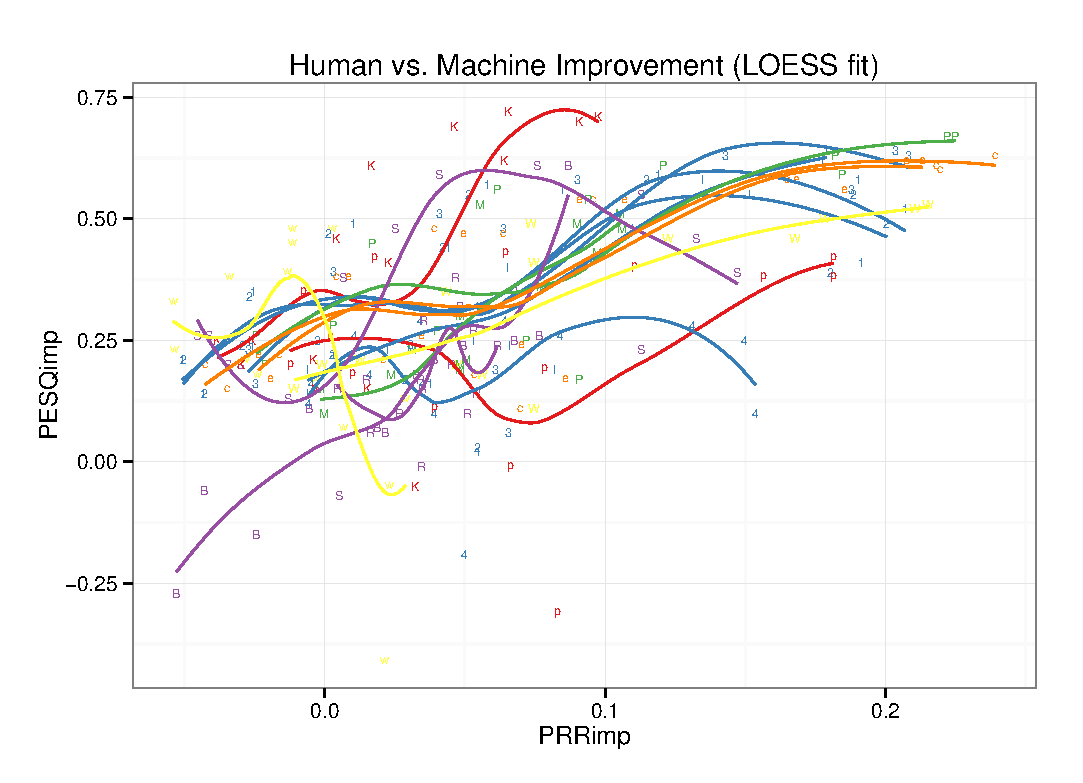
\includegraphics[width=1\textwidth]{fig/R/dir/lit/HumanMachineAllLOESS}

}

\subfloat[\label{fig:Direct-PESQ-PRR-LM}\acl{LM} fit]{\includegraphics[width=0.8\textwidth]{fig/R/dir/lit/HumanMachineAllLM}\includegraphics[width=0.2\textwidth]{fig/R/dir/lit/HumanMachineAllLegend}

}\protect\caption{\label{fig:Direct-PESQ-PRR}Direct comparison of human (\acs{PESQ})
vs. machine (\acs{PRR}) quality improvement}
\end{figure}


Additionally, a Pearson's correlation table was formed over a number
of the evaluation measures, depicted in the correlogram in \figref{litResCorr}.
The sparsity in this figure is due to the limited amount of pre-existing
data.

\begin{minipage}[t]{1\columnwidth}%
\begin{shaded}%

\subsubsection*{Correlograms}

A correlogram is a plot designed to allow the reader to quickly observe
the relationship between a number of variables. In the correlograms
included within this thesis, the leading diagonal shows the variable
name corresponding to that row and column. The upper panels display
a scatterplot where the y-axis represents the the variable of the
panel's row, and the x-axis represents the variable of the panel's
column. The lower panels show the Pearson's correlation of the two
variable the panel intersects, the 95\% confidence interval. Additionally,
lower panels are highlighted in red for negative correlations and
blue for positive correlations, with the darkness indicating magnitude.

So the darker shaded panels in the lower half indicate variables that
are strongly correlated, and allows the reader to quickly establish
which relationships are meaningful. The relationship can be visually
confirmed by checking the scatterplot in the upper half. The relationships
can then be further investigated by forming further plots of the variables
of interest.\end{shaded}%
\end{minipage}

\begin{figure}[H]
\noindent \begin{centering}
\includegraphics[width=1\textwidth]{fig/R/cor/litResCorrgram}
\par\end{centering}

\protect\caption{\label{fig:litResCorr}Correlogram of some of the evaluation measures
assessed in existing data}
\end{figure}


These results showed a general, positive correlation between \ac{PESQ}
improvement and \ac{PRR} improvement, and by extension between \ac{HR}
and \ac{MR}. The level of correlation appeared to be somewhat low,
however comparison with \figref{litResCorr} indicated a correlation
between \lstinline!PESQimp! and \lstinline!PRRimp! of approximately
0.58. The same figure indicated a correlation between \lstinline!PESQraw!
and \lstinline!MOSraw! of approximately 0.65, which were measures
that have been shown to be correlated in literature \citep{Kitawaki2007,Rix2003,Rix2001}.
Therefore, the correlation of 0.58 between \ac{PESQ} improvement
and \ac{PRR} improvement can be considered significant. \figref{litResCorr}
Also indicated a very high correlation between the raw \ac{PESQ}
result and \ac{PRR}.

These observations indicated a good correlation between human recognition
(\ac{MOS}) and human estimated recognition (\ac{PESQ}); as well
as a strong correlation between human estimated recognition (\ac{PESQ})
and machine recognition (\ac{PRR} correctness). Therefore, it was
inferred that there is likely a good correlation between human recognition
and machine recognition.

A number of further observations were drawn from \figref{Direct-PESQ-PRR},
and are highlighted in \cref{fig:direct-klt-mband,fig:direct-klt-pklt,fig:direct-pklt-logmmse-spu-4,fig:direct-highcorr}.

Results found using the \ac{LOESS} fitted method, shown in \figref{Direct-PESQ-PRR-LOESS}
indicated that the data could be approximated by a linear model: the
\ac{LOESS} fitted lines were, in most cases, approximately linear.
The results for Wiener algorithms were a notable exception, with a
non-linear variation, even when the outliers are ignored. Overall,
the \ac{LM} fit in \figref{Direct-PESQ-PRR-LM} is accepted to be
accurate. The linear model was used in the following observations.

\begin{figure}[h]
\noindent \begin{centering}
\includegraphics[width=0.8\textwidth]{fig/R/dir/lit/KLT-MBAND/HumanMachineAllLM}\includegraphics[width=0.2\textwidth]{fig/R/dir/lit/HumanMachineAllLegend}
\par\end{centering}

\protect\caption{\label{fig:direct-klt-mband}Direct comparison of \acs{PESQ} vs.
\acs{PRR} highlighting \acs{KLT} and \acs{MBAND}}
\end{figure}


Despite the high correlation between \ac{PESQ} and \ac{PRR} observed,
there is still evidence to show that algorithms' performances vary
depending on the performance measure used. For example, highlighted
in \figref{direct-klt-mband} are two algorithms, the \ac{KLT} method
and the \ac{MBAND} method, that exhibited similar performances when
evaluated by \ac{PRR}, a machine measure. However, when evaluated
by a human perceptual method, \ac{PESQ}, the \ac{KLT} method clearly
performed better. In fact, the \ac{KLT} method exhibited one of the
best performances seen on the \ac{PESQ} scale, whereas the \ac{MBAND}
method was the worst performer on this scale, exhibiting loss in perceptual
quality, as indicated by the negative performance.

\begin{figure}[h]
\noindent \begin{centering}
\includegraphics[width=0.8\textwidth]{fig/R/dir/lit/KLT-pKLT/HumanMachineAllLM}\includegraphics[width=0.2\textwidth]{fig/R/dir/lit/HumanMachineAllLegend}
\par\end{centering}

\protect\caption{\label{fig:direct-klt-pklt}Direct comparison of \acs{PESQ} vs. \acs{PRR}
highlighting \acs{KLT} and \acs{pKLT}}
\end{figure}


\figref{direct-klt-pklt} shows the \ac{PESQ} vs. \ac{PRR} improvement
with the \ac{KLT} and \ac{pKLT} algorithm performances highlighted.
This was noted as an example of two very similar algorithms, with
varying performance between \ac{HR} and \ac{MR} results. The \ac{KLT}
results exhibited better performance for a human listener, as the
points laid higher on the y-axis, whereas the \ac{pKLT} results exhibited
better performance for a machine recogniser, as the points laid higher
on the x-axis.

Such results support the proposition that some algorithms are inherently
suited either towards human or machine listeners. However, this shows
that such distinction is not necessarily related to the algorithm
class, since the \ac{KLT} and \ac{pKLT} algorithms belonged to the
same \ac{KLT} class, but produced different results.

\begin{figure}[h]
\noindent \begin{centering}
\includegraphics[width=0.8\textwidth]{fig/R/dir/lit/pKLT-logMMSE-SPU-4/HumanMachineAllLM}\includegraphics[width=0.2\textwidth]{fig/R/dir/lit/HumanMachineAllLegend}
\par\end{centering}

\protect\caption{\label{fig:direct-pklt-logmmse-spu-4}Direct comparison of \acs{PESQ}
vs. \acs{PRR} highlighting \acs{logMMSE} \acs{SPU} and \acs{pKLT}}
\end{figure}


The \ac{pKLT} and \ac{logMMSE-SPU-4} algorithms were observed to
show reasonable improvement in \ac{PRR} as the \ac{SNR} increased,
but little to no improvement in \ac{PESQ}. This is highlighted in
\figref{direct-pklt-logmmse-spu-4}, and is apparent by the near-zero
gradient. These algorithms likely introduce distortions into the signal
in the process of enhancement that the \ac{ASR} algorithm was immune
to, however would be distracting to a human and therefore performed
badly under the \ac{PESQ} evaluation.

\begin{figure}[h]
\noindent \begin{centering}
\includegraphics[width=0.8\textwidth]{fig/R/dir/lit/MMSE-SPU-STSA-wcosh-STSA-weuclid-logMMSE-SPU-3/HumanMachineAllLM}\includegraphics[width=0.2\textwidth]{fig/R/dir/lit/HumanMachineAllLegend}
\par\end{centering}

\protect\caption{\label{fig:direct-highcorr}\acs{STSA-wcosh}, \acs{STSA-weuclid}
and \acs{logMMSE-SPU-3}}
\end{figure}


The final observation drawn from \figref{Direct-PESQ-PRR} is highlighted
in \figref{direct-highcorr}, which shows the \ac{MMSE-SPU}, \ac{STSA-wcosh},
\ac{STSA-weuclid} and \ac{logMMSE-SPU-3} algorithms. These algorithms
show a high, positive correlation with one another, as well as exhibiting
the best results measured for both \ac{PESQ} and \ac{PRR}. The evidence
suggests such a response is the ideal case, and that there exists
algorithms which are capable of performing well for both human and
machine recognisers.

Therefore, existing data showed that in general there was a correlation
between enhancement for \ac{HR} and \ac{MR}. However, one cannot
be used as a reliable measure of the other, as there are notable exceptions
where enhancement for one class did not show enhancement for the other.

\clearpage{}


\subsection{Independent Investigation into \acl{HR} and \acl{MR}\label{sub:Independent-Investigation-Res}}

An independent investigation was conducted in which a number of enhancement
algorithms were implemented. The enhanced waveforms were then analysed
using a number of enhancement methods, covering both \ac{HR} and
\ac{MR}. The goal was to determine the correlation between evaluation
measures of enhancement, specifically those for \ac{HR} with those
for \ac{MR}.

These results corresponded to algorithms listed in \tabref{Algorithms},
\textit{\nameref{tab:Algorithms}} and the evaluation measures outlined
in \subsecref{Independent-Investigation-Meth}, \textit{\nameref{sub:Independent-Investigation-Meth}}.
A correlogram of the results was formed in \figref{my-Corr} to give
an overview of the results and how measures correlated with one another.
In this figure:
\begin{itemize}
\item the \lstinline!utterances! and \lstinline!phonemes! rows/columns
correspond to the training given to the enhancement algorithm;
\item ``Imp'' refers to improvement comparatively with the signal before
enhancement, i.e., \lstinline!pesqImp! refers to the \ac{PESQ} score
after enhancement minus the \ac{PESQ} score before enhancement;
\item \lstinline!MOSle! refers to the \ac{MOS} listening effort scale
\citep{InternationalTelecommunicationUnion1996};
\item \lstinline!CMOS! refers to the comparative \ac{MOS};
\item \lstinline!PRRcorr! refers to the \ac{PRR} measured as the percentage
correct, or \ac{PRR} correctness;
\item \lstinline!PRRacc! refers the the \ac{PRR} measures as the accuracy,
defined as the number of correct phonemes minus the number of deletions,
substitutions and insertions, divided by the number of phonemes; and
\item \lstinline!segSNR! refers to the segmental \ac{SNR}.
\end{itemize}
The results for the various evaluation measures are given in \cref{fig:my-PESQ,fig:my-PESQ-imp,fig:my-segSNR,fig:my-segSNR-imp,fig:my-PRRcorr,fig:my-MOS,fig:my-MOSle,fig:my-CMOS,fig:my-PRRcorr-imp,fig:my-PRRacc,fig:my-PRRacc-imp}.
These plots also show box plots of the five-point summaries of the
results. These results were obtained to be used in investigating the
correlation between \ac{HR} and \ac{MR} and also to assess the performance
of the proposed changes to the enhancement algorithms outlined in
\secref{Develop-Phoneme-Dependent}. The changes proposed in \subsecref{Phoneme-Training}
are implemented in the algorithms \lstinline[breaklines=true]!phonemeIDBM!,
\lstinline[breaklines=true]!phonemeMMSE!, \lstinline[breaklines=true]!phonemeMohammadiaOnline!
and \lstinline[breaklines=true]!phonemeMohammadiaSupervised!. The
changes proposed in \subsecref{Phoneme-Base} are implemented in the
algorithms \lstinline[breaklines=true]!phonemeModifiedOnline! and\inputencoding{latin1}{}\linebreak{}
\inputencoding{latin9}\lstinline[breaklines=true]!phonemeModifiedSupervised!.


\subsubsection*{Observations}

During the \ac{MOS} tests it was noted that most participants complained
that occasionally a signal would not play. Upon further investigation
it was determined that the signal was in fact playing, but consisted
of silence. Subjects were instructed to continue answering the questions
as they were worded, and thus these signals were given the minimum
scores. This is reflected in \cref{fig:my-MOS,fig:my-MOSle,fig:my-CMOS},
where the ideal binary mask algorithms scored poorly.

\begin{figure}[h]
\noindent \begin{centering}
\includegraphics[width=1\textwidth]{fig/R/dir/my/corr}
\par\end{centering}

\protect\caption{\label{fig:my-Corr}Correlogram of results of independent investigation}
\end{figure}


\begin{figure}[p]
\noindent \begin{centering}
\includegraphics[angle=90,width=1\textwidth,height=0.95\textheight]{fig/R/my/pesq}
\par\end{centering}

\protect\caption{\label{fig:my-PESQ}\acs{PESQ} results of independent investigation}
\end{figure}


\begin{figure}[p]
\noindent \begin{centering}
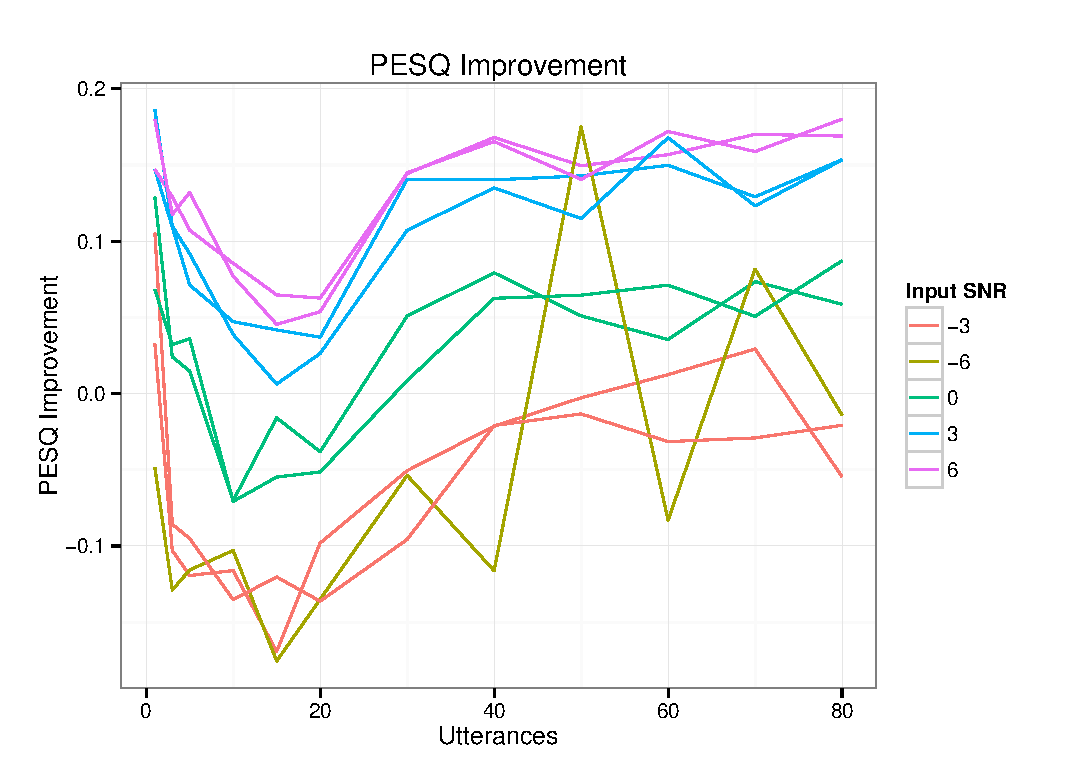
\includegraphics[angle=90,width=1\textwidth,height=0.95\textheight]{fig/R/my/pesqImp}
\par\end{centering}

\protect\caption{\label{fig:my-PESQ-imp}Improvement in \acs{PESQ} score due to enhancement}
\end{figure}


\begin{figure}[h]
\noindent \begin{centering}
\includegraphics[angle=90,width=1\textwidth,height=0.95\textheight]{fig/R/my/segSNR}
\par\end{centering}

\protect\caption{\label{fig:my-segSNR}Segmental \acs{SNR} results of independent
investigation}
\end{figure}


\begin{figure}[h]
\noindent \begin{centering}
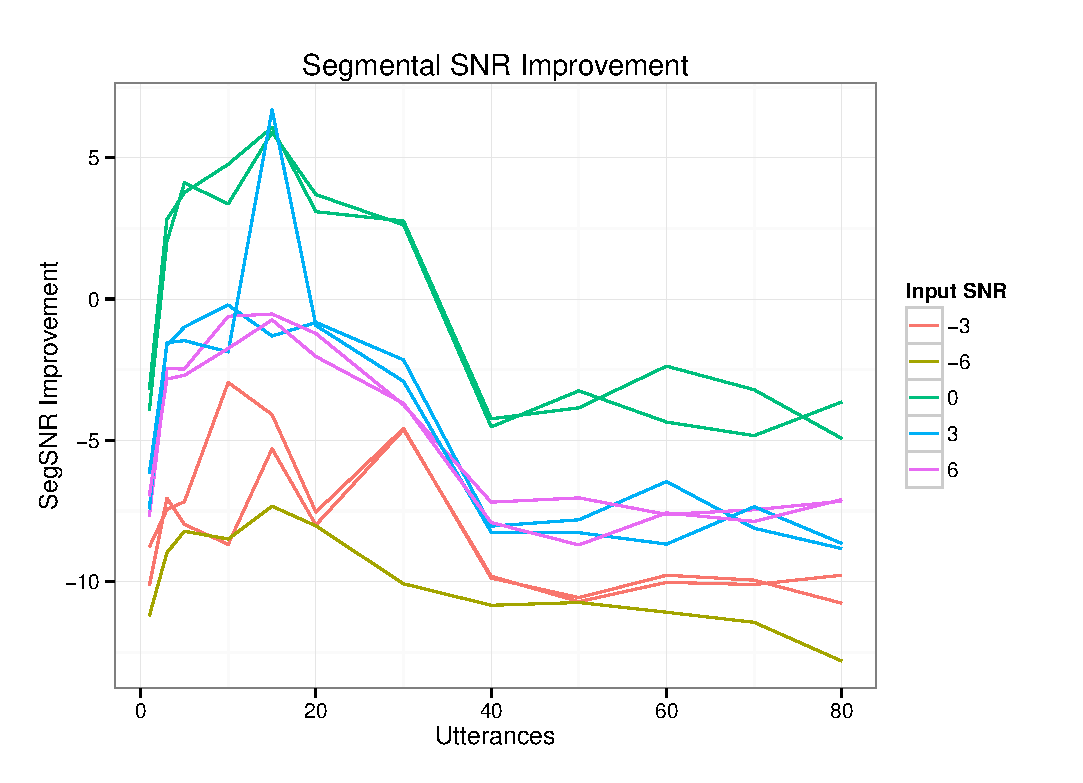
\includegraphics[angle=90,width=1\textwidth,height=0.95\textheight]{fig/R/my/segSNRImp}
\par\end{centering}

\protect\caption{\label{fig:my-segSNR-imp}Improvement in segmental \acs{SNR} score
due to enhancement}
\end{figure}


\begin{figure}[h]
\noindent \begin{centering}
\includegraphics[angle=90,width=1\textwidth,height=0.95\textheight,keepaspectratio]{fig/R/my/MOS}
\par\end{centering}

\protect\caption{\label{fig:my-MOS}\acs{MOS} results of independent investigation}
\end{figure}


\begin{figure}[h]
\noindent \begin{centering}
\includegraphics[angle=90,width=1\textwidth,height=0.95\textheight,keepaspectratio]{fig/R/my/MOSle}
\par\end{centering}

\protect\caption{\label{fig:my-MOSle}Listening effort \acs{MOS} results of independent
investigation}
\end{figure}


\begin{figure}[h]
\noindent \begin{centering}
\includegraphics[angle=90,width=1\textwidth,height=0.95\textheight,keepaspectratio]{fig/R/my/CMOS}
\par\end{centering}

\protect\caption{\label{fig:my-CMOS}Comparative \acs{MOS} results of independent
investigation}
\end{figure}


\begin{figure}[h]
\noindent \begin{centering}
\includegraphics[angle=90,width=1\textwidth,height=0.95\textheight,keepaspectratio]{fig/R/my/PRRcorr}
\par\end{centering}

\protect\caption{\label{fig:my-PRRcorr}\acs{PRR} correctness results of independent
investigation}
\end{figure}


\begin{figure}[h]
\noindent \begin{centering}
\includegraphics[angle=90,width=1\textwidth,height=0.95\textheight,keepaspectratio]{fig/R/my/PRRcorrImp}
\par\end{centering}

\protect\caption{\label{fig:my-PRRcorr-imp}Improvement in \acs{PRR} correctness due
to enhancement}
\end{figure}


\begin{figure}[h]
\noindent \begin{centering}
\includegraphics[angle=90,width=1\textwidth,height=0.95\textheight,keepaspectratio]{fig/R/my/PRRacc}
\par\end{centering}

\protect\caption{\label{fig:my-PRRacc}\acs{PRR} accuracy results of independent investigation}
\end{figure}


\begin{figure}[h]
\noindent \begin{centering}
\includegraphics[angle=90,width=1\textwidth,height=0.95\textheight,keepaspectratio]{fig/R/my/PRRaccImp}
\par\end{centering}

\protect\caption{\label{fig:my-PRRacc-imp}Improvement in \acs{PRR} accuracy due to
enhancement}
\end{figure}


\clearpage{}


\subsubsection*{On the relationship between \acs{PESQ} and \acs{MOS}}

In \figref{my-Corr}, the correlation between \ac{PESQ} and the various
\ac{MOS} measures was shown to be very low. This was a surprising
results as it has generally been determined in literature that the
two correlate well \citep{Kitawaki2007,Rix2003,Rix2001}, albeit with
some exceptions \citep{Liu2006}. This correlation is highlighted
in \figref{my-pesq-mos-with-idbm}.

\begin{figure}[bh]
\subfloat[\label{fig:my-pesq-mos-with-idbm}With the ideal binary mask]{\includegraphics[width=0.5\textwidth]{fig/R/pair/my/pesq-mos}

}\subfloat[\label{fig:my-pesq-mos-without-idbm}Without the ideal binary mask]{\includegraphics[width=0.5\textwidth]{fig/R/pair/my/pesq-mos_no-IDBM}

}

\includegraphics[width=1\textwidth]{fig/R/pair/my/pesq-mos_leg}

\protect\caption{\label{fig:my-pesq-mos}Scatterplot of \acs{PESQ} vs. \acs{MOS}
results}
\end{figure}


The greatest deviation to the correlation between \ac{PESQ} and \ac{MOS}
was due to the results of the ideal binary mask algorithms (\lstinline!IDBM!
and \lstinline!phonemeIDBM!). It was also noted that the ideal binary
mask algorithms performed very poorly overall on the subjective \ac{MOS}
scales in \cref{fig:my-MOS,fig:my-MOSle,fig:my-CMOS}. Furthermore,
ideal binary mask algorithms had a very high variation in \ac{PESQ}
performance in \figref{my-PESQ}, receiving both the highest and the
lowest scores of all tests on the \ac{PESQ} scale. Therefore, it
was suspected that the ideal binary mask corrupted speech in such
a way that was not detected by the \ac{PESQ} algorithm.

It was found that when the ideal binary mask algorithm data was omitted
the correlation between the \ac{PESQ} and \ac{MOS} increased, as
demonstrated in \figref{my-pesq-mos-without-idbm}. This indicated
there were specific occurrences for which the relationship between
\ac{PESQ} and \ac{MOS} demonstrated in literature do not hold, i.e.,
distortions detectable by human hearing but not by the \ac{PESQ}
algorithm.

The correlation of 0.173 between \ac{PESQ} and \ac{MOS} is still
low. This was likely in part due to the low sample size used, with
only ten subjects. Also, the standard \ac{MOS} measure is highly
subjective. This was possibly due to listeners not having a reference
for scoring. Comparative \ac{MOS} is therefore advantageous in that
it asks the listener to rate the difference between two recordings,
so the listener has a reference. \figref{my-pesqimp-cmos} shows similar
results to \figref{my-pesq-mos}, however instead considers the \ac{PESQ}
improvement as opposed to the enhanced \ac{PESQ} score, and considers
the comparative \ac{MOS} instead of the \ac{MOS}. \ac{PESQ} improvement
was used due to it being more similar to comparative \ac{MOS}, as
these both measure the differential improvement (or distortion).

\begin{figure}[h]
\subfloat[\label{fig:my-pesqimp-cmos-with-idbm}With the ideal binary mask]{\includegraphics[width=0.5\textwidth]{fig/R/pair/my/pesqimp-cmos}

}\subfloat[\label{fig:my-pesqimp-cmos-without-idbm}Without the ideal binary
mask]{\includegraphics[width=0.5\textwidth]{fig/R/pair/my/pesqimp-cmos_no-IDBM}

}

\includegraphics[width=1\textwidth]{fig/R/pair/my/pesqimp-cmos_leg}

\protect\caption{\label{fig:my-pesqimp-cmos}Scatterplot of \acs{PESQ} improvement
vs. comparative \acs{MOS} results}
\end{figure}


When, for the same reason as stated above, the ideal binary mask results
were omitted (\figref{my-pesqimp-cmos-without-idbm}) the correlation
rose to 0.436, which represented a fair correlation and was considered
significant. Also of note were the \lstinline!phonememohammadiaOnline!
results in \figref{my-pesqimp-cmos-without-idbm} that scored between
1 and 2 on the comparative \ac{MOS} test, but between -0.5 and -1
on the \ac{PESQ} improvement scale. A difference of 1 on the \ac{PESQ}
scale represents a significant distortion, however these particular
results were rated by human listeners to be somewhere between ``slightly
better'' and ``better''.

Results indicated that the \ac{PESQ} scale may be better considered
to be a rough indicator for human perception of enhancement, rather
than a direct measure of it. Circumstances in which human hearing
detected significant distortions have not been evaluated as so on
the \ac{PESQ} scale. However, not enough \ac{MOS} test subjects
were included in testing to conclusively evaluate the reliability
of \ac{PESQ}.

Results also indicated that comparative \ac{MOS} may be a less subjective
measure than regular \ac{MOS}, due to the inherent use of a reference.
Comparative \ac{MOS} also was found to lend itself to measuring enhancement,
so is a better candidate than regular \ac{MOS} for measuring enhancement.


\subsubsection*{On the relationship between similar measures}

The \ac{MOS} evaluation measures, \lstinline!MOS!, \lstinline!MOSle!,
and \lstinline!CMOS!, had a strong correlation with one-another in
\figref{my-Corr}, all at approximately 90\%. This was expected between
similar measures. However, it was noted that the same was not true
for the \ac{PRR} measures, where the correlation between the correctness
(\lstinline!PRRcorr!) and the accuracy (\lstinline!PRRacc!) was
found to be negative. This highlighted the balance between an under-trained
and under-discriminative algorithm, which may detect a high number
of correct phonemes (high correctness) but poorly reduce noise and
therefore recognise extra incorrect phonemes (low accuracy); and an
over-trained and over-discriminative algorithm, which may detect a
lower number of correct phonemes (low correctness) but effectively
reduce noise and therefore have minimal false positiveness(increased
accuracy).


\subsubsection*{On the relationship between \acl{HR} and \acl{MR}}

\figref{my-Corr} showed a significant positive correlation between
the various \ac{MOS} measures (\lstinline!MOS!, \lstinline!MOSle!,
and \lstinline!CMOS!) and the \ac{PRR} measured as correctness (\lstinline!PRRcorr!).
However, the figure also shows an almost as significant negative correlation
between the various \ac{MOS} measures and the \ac{PRR} measured
as accuracy (\lstinline!PRRacc!).

\begin{figure}[h]
\subfloat[\label{fig:mos-prrcorr}\acs{MOS} vs. \acs{ASR} correctness]{\includegraphics[width=0.5\textwidth]{fig/R/pair/byTest/mos-prrcorr}

}\subfloat[\label{fig:mos-prracc}\acs{MOS} vs. \acs{ASR} accuracy]{\includegraphics[width=0.5\textwidth]{fig/R/pair/byTest/mos-prracc}

}

\subfloat[\label{fig:cmos-prrcorrimp}Comparative \acs{MOS} vs. \acs{ASR}
correctness improvement]{\includegraphics[width=0.5\textwidth]{fig/R/pair/byTest/cmos-prrcorrimp}

}\subfloat[\label{fig:cmos-prraccimp}Comparative \acs{MOS} vs. \acs{ASR} accuracy
improvement]{\includegraphics[width=0.5\textwidth]{fig/R/pair/byTest/cmos-prraccimp}

}

\noindent \begin{centering}
\includegraphics[width=0.6\linewidth]{fig/R/pair/byTest/mos-prr-leg}
\par\end{centering}

\protect\caption{\label{fig:hr-mr}Scatterplot of \acs{HR} and \acs{MR} measures,
highlighting test conditions}
\end{figure}


\figref{hr-mr} show scatterplots measuring human performance on the
y-axis and machine improvement on the x-axis, and highlighting in
colour the test conditions.

\cref{fig:mos-prrcorr,fig:cmos-prrcorrimp} measured the \ac{PRR}
correctness. \figref{mos-prrcorr} also shows the relative density
of points, revealing that certain test conditions are clustered outliers
and that the correlation might otherwise have been higher. It was
seen that tests where there was one competing speaker of the same
sex, highlighted in red, were characterised by a mid-range \ac{MOS}
result, but a high correctness \ac{PRR}. This indicated the \ac{ASR}
system was able to still detect the \ac{SoI}'s voice, however a human
listener scored the signal as average. This also supported previous
observations indicating certain systematic conditions for which the
correlation between \ac{HR} and \ac{MR} deviate.

\cref{fig:mos-prracc,fig:cmos-prraccimp} measured the \ac{PRR} accuracy.
These figures showed that once the \ac{ASR} phoneme insertions are
taken into account the correlation between \ac{HR} and \ac{MR} no
longer held.

\figref{hr-mr-alg} shows the same data as \cref{fig:cmos-prrcorrimp,fig:cmos-prraccimp},
but with colour highlighting the enhancement algorithm as opposed
to the test conditions. A very interesting observation made was the
clustered performance of the ideal binary mask (\lstinline!IDBM!)
and phoneme-dependent ideal binary mask (\lstinline!phonemeIDBM!)
in the lower right corner, especially under accuracy \ac{PRR}. These
algorithms achieved the highest \ac{PRR} accuracy score of any algorithm,
some approaching a 30\% accuracy increase, despite performing poorly
on all \ac{HR} and statistical measures. These results were also
noted by observing the ideal binary mask algorithms performance in
\cref{fig:my-PRRacc,fig:my-PRRacc-imp}, and is reflected on by the
observation made in \subsecref{Independent-Investigation-Res}.

\begin{figure}[h]
\subfloat[\label{fig:cmos-prrcorrimp-alg}Comparative \acs{MOS} vs. \acs{ASR}
correctness improvement]{\includegraphics[width=0.5\textwidth]{fig/R/pair/byAlg/cmos-prrcorrimp}

}\subfloat[\label{fig:cmos-prraccimp-alg}Comparative \acs{MOS} vs. \acs{ASR}
accuracy improvement]{\includegraphics[width=0.5\textwidth]{fig/R/pair/byAlg/cmos-prraccimp}

}

\noindent \begin{centering}
\includegraphics[width=0.9\linewidth]{fig/R/pair/byAlg/mos-prr-leg}
\par\end{centering}

\protect\caption{\label{fig:hr-mr-alg}Scatterplot of \acs{HR} and \acs{MR} measures,
highlighting enhancement algorithm}
\end{figure}


The explanation given for this behaviour was that the ideal binary
mask algorithms were effective in eliminating the competing noise,
and thus reducing false insertions. However, in the process these
algorithms distort the signal, severely for humans, thereby drastically
reducing human intelligibility, and also causing the loss in correctness
\ac{PRR} exhibited in \figref{my-PRRcorr-imp}.

Therefore, the results of the independent investigation into \ac{HR}
vs. \ac{MR} perception of speech enhancement agreed with the results
of the investigation into existing data. It has been determined that
that in general there was a correlation between enhancement for \ac{HR}
and \ac{MR}. However, one cannot be used as a reliable measure of
the other, as there are notable exceptions where enhancement for one
class did not show enhancement for the other.


\section{Assessing \acl{NMF} Algorithm Training}

The following are the results of investigations attempting to answer
Research Question \ref{enu:ResQ2}, \textit{\RQtwo{}}


\subsection{Investigating Training Requirements}

The results of the experiments proposed in \subsecref{Investigating-Training-Req}
are given in this section. \cref{fig:vary-train-pesq,fig:vary-train-mos,fig:vary-train-mosle,fig:vary-train-cmos,fig:vary-train-prrcorr,fig:vary-train-prracc,fig:vary-train-segsnr}
show the \ac{PESQ}, \ac{MOS}, \ac{MOS} listening effort, comparative
\ac{MOS}, \ac{PRR} correctness and \ac{PRR} accuracy results of
the \ac{BNMF} algorithm developed by \citet{mohammadiha2013supervised}
as a function of the number of utterances used in training.

Plots in \cref{fig:vary-train-pesq,fig:vary-train-mos,fig:vary-train-mosle,fig:vary-train-cmos,fig:vary-train-prrcorr,fig:vary-train-prracc,fig:vary-train-segsnr}
each are arranged with the number of trained utterances on the x-axis
and test score on the y-axis. Furthermore, the plots are arranged
in a grid with rows corresponding to the enhancement algorithm and
columns corresponding to the test. Test labels give information on
the speaker ID and in brackets the sex of both the SoI, and the speakers
used to form the noise babble. Finally, series colour represents the
\ac{SNR} used for the test data, and the line type is dashed when
representing the score of the dirty signal before enhancement. The
R script used to form these plots is given in \lstref{trainReq}.

\begin{figure}[p]
\noindent \begin{centering}
\includegraphics[angle=90,width=1\textwidth,height=0.95\textheight,keepaspectratio]{fig/R/train/pesq}
\par\end{centering}

\protect\caption{\label{fig:vary-train-pesq}\acs{PESQ} results of \acs{BNMF} algorithm
as training is increased}
\end{figure}


\begin{figure}[p]
\noindent \begin{centering}
\includegraphics[angle=90,width=1\textwidth,height=0.95\textheight,keepaspectratio]{fig/R/train/MOS}
\par\end{centering}

\protect\caption{\label{fig:vary-train-mos}\acs{MOS} results of \acs{BNMF} algorithm
as training is increased}
\end{figure}


\begin{figure}[p]
\noindent \begin{centering}
\includegraphics[angle=90,width=1\textwidth,height=0.95\textheight,keepaspectratio]{fig/R/train/mosle}
\par\end{centering}

\protect\caption{\label{fig:vary-train-mosle}\acs{MOS} listening effort results of
\acs{BNMF} algorithm as training is increased}
\end{figure}


\begin{figure}[p]
\noindent \begin{centering}
\includegraphics[angle=90,width=1\textwidth,height=0.95\textheight,keepaspectratio]{fig/R/train/CMOS}
\par\end{centering}

\protect\caption{\label{fig:vary-train-cmos}Comparative \acs{MOS} results of \acs{BNMF}
algorithm as training is increased}
\end{figure}


\begin{figure}[p]
\noindent \begin{centering}
\includegraphics[angle=90,width=1\textwidth,height=0.95\textheight,keepaspectratio]{fig/R/train/prrcorr}
\par\end{centering}

\protect\caption{\label{fig:vary-train-prrcorr} \acs{PRR} correctness results of
\acs{BNMF} algorithm as training is increased}
\end{figure}


\begin{figure}[p]
\noindent \begin{centering}
\includegraphics[angle=90,width=1\textwidth,height=0.95\textheight,keepaspectratio]{fig/R/train/prracc}
\par\end{centering}

\protect\caption{\label{fig:vary-train-prracc} \acs{PRR} accuracy results of \acs{BNMF}
algorithm as training is increased}
\end{figure}


\begin{figure}[p]
\noindent \begin{centering}
\includegraphics[angle=90,width=1\textwidth,height=0.95\textheight,keepaspectratio]{fig/R/train/segSNR}
\par\end{centering}

\protect\caption{\label{fig:vary-train-segsnr}Segmental \acs{SNR} results of \acs{BNMF}
algorithm as training is increased}
\end{figure}


\clearpage{}

All measurements, for all enhancement methods, tended to agree that
there was no particular correlation between training and performance.
Before tests were performed, it was hypothesised that increasing the
number of utterances provided as training would allow the algorithm
to produce a better model, with more data to learn from. However,
the number of utterances provided for training of the online \ac{BNMF}
algorithm in \figref{vary-train-pesq} had no significant impact on
\ac{PESQ} performance. This conclusions is supported by \figref{my-PRRcorr-imp},
showing no significant correlation between \lstinline!utterances!
and any of the test measures, with the exception of \lstinline!prrCorr!.
However, \figref{vary-train-prrcorr} showed no evidence of a correlation
between the number of utterances for training and the \ac{PRR} correctness.

A notable observation was that for the human and machine measures,
those in \cref{fig:vary-train-pesq,fig:vary-train-mos,fig:vary-train-mosle,fig:vary-train-cmos,fig:vary-train-prrcorr,fig:vary-train-prracc},
there was a high variability in performance for ten or less utterances.
This indicated that the algorithms were under-trained when 10 or less
utterances were used.

It was also noted that in some cases, the performance was better in
the under-trained case, for example in \figref{vary-train-pesq} for
\lstinline!mohammadiaSupervised! with the\inputencoding{latin1}{}\linebreak{}
\inputencoding{latin9}\lstinline!c3f(m)+c3c(f)+c35(m)! noise type.
This indicated that the training method used was not optimal. This
provided further reason for implementing the phoneme-dependent algorithms,
in an attempt to optimise the training by reducing the training data
size whilst maximising the amount of voice information.

Thus is was shown that approximately 10 to 20 utterances was required
to sufficiently train the online and supervised \ac{BNMF} algorithms,
but increasing beyond that level had little effect. It has also been
shown that this type of training is not optimal, showing opportunity
for phoneme-dependent training.

\clearpage{}


\section{Phoneme-Dependent Variation Performance}

The results of the phoneme-dependent \textbf{training} algorithm proposed
in \subsecref{Phoneme-Training} and the phoneme-dependent \textbf{base}
algorithm proposed in \subsecref{Phoneme-Base} are given in this
section.

The typical spectrograms of the drawn phonemes are given in \figref{drawn-phoneme-spectrogram},
showing the frequency characteristics of each phoneme. The voiced
phonemes were seen to contain lower frequency components and the voiceless
phonemes contained higher frequency components as expected. The differences
in phonemes was clear and identifiable, indicating that the method
worked as intended. One issue noted was that voiceless stops, were
too short and were occasionally missed. A noted example was in the
first two phoneme samples in \figref{mos-comparison-phn-1}, which
were /\textit{p}/ and /\textit{t}/. For such phonemes, high frequency
components would have been expected, but mostly silence present with
some lower frequency components. The same phonemes in \figref{mos-comparison-phn-5}
revealed that only two out of the ten phoneme slices contained the
expected high frequency components. However, these kind of errors
were expected and is one of the reasons that the number of slices
per phoneme was varied, which is discussed in \subsecref{Varying-Phns}.

There was little to no visual difference after 50 to 100 phoneme samples
were drawn. Additionally, the length of recordings stopped increasing
around this point. After this the saturation point for the recordings
used was reached, where there were not enough phoneme occurrences
to support having more samples. So the tests done for more samples
per phoneme than 100 were, for the most part, redundant.

The performance of the phoneme-dependant algorithms have already been
given in \cref{fig:my-PESQ,fig:my-PESQ-imp,fig:my-segSNR,fig:my-segSNR-imp,fig:my-PRRcorr,fig:my-MOS,fig:my-MOSle,fig:my-CMOS,fig:my-PRRcorr-imp,fig:my-PRRacc,fig:my-PRRacc-imp},
since these algorithms were also considered in the previous investigation.

Additionally given are plots comparing the performance of algorithms
without modification against those with phoneme-dependent modification.
These are given in \cref{fig:pesq-comparison-phn,fig:mos-comparison-phn,fig:mosle-comparison-phn,fig:cmos-comparison-phn,fig:prrcorr-comparison-phn,fig:prrcorrimp-comparison-phn,fig:prracc-comparison-phn,fig:prraccimp-comparison-phn,fig:segsnr-comparison-phn,fig:segsnrimp-comparison-phn}.
In these plots, the x-axis measures the performance of the original
algorithm, and the y-axis measures performance of the modified algorithm.
Therefore, any points lying above the diagonal line show better performance
for the modified algorithm, and below the line show better performance
for the original algorithm.

The phoneme dependent training data changes proposed in \subsecref{Phoneme-Training}
are implemented in the algorithms \lstinline[breaklines=true]!phonemeIDBM!,
\lstinline[breaklines=true]!phonemeMMSE!, \lstinline[breaklines=true]!phonemeMohammadiaOnline!
and\linebreak{}
\lstinline[breaklines=true]!phonemeMohammadiaSupervised! in \cref{fig:my-PESQ,fig:my-PESQ-imp,fig:my-segSNR,fig:my-segSNR-imp,fig:my-PRRcorr,fig:my-MOS,fig:my-MOSle,fig:my-CMOS,fig:my-PRRcorr-imp,fig:my-PRRacc,fig:my-PRRacc-imp},
and are labelled ``Phoneme Training'' in \cref{fig:pesq-comparison-phn,fig:mos-comparison-phn,fig:mosle-comparison-phn,fig:cmos-comparison-phn,fig:prrcorr-comparison-phn,fig:prrcorrimp-comparison-phn,fig:prracc-comparison-phn,fig:prraccimp-comparison-phn,fig:segsnr-comparison-phn,fig:segsnrimp-comparison-phn}.

The phoneme dependent base matrix changes proposed in \subsecref{Phoneme-Base}
are implemented in the algorithms \lstinline[breaklines=true]!phonemeModifiedOnline!
and \lstinline[breaklines=true]!phonemeModifiedSupervised! in \cref{fig:my-PESQ,fig:my-PESQ-imp,fig:my-segSNR,fig:my-segSNR-imp,fig:my-PRRcorr,fig:my-MOS,fig:my-MOSle,fig:my-CMOS,fig:my-PRRcorr-imp,fig:my-PRRacc,fig:my-PRRacc-imp},
and are labelled ``Phoneme Dictionary (Modified)'' in \cref{fig:pesq-comparison-phn,fig:mos-comparison-phn,fig:mosle-comparison-phn,fig:cmos-comparison-phn,fig:prrcorr-comparison-phn,fig:prrcorrimp-comparison-phn,fig:prracc-comparison-phn,fig:prraccimp-comparison-phn,fig:segsnr-comparison-phn,fig:segsnrimp-comparison-phn}.

\begin{figure}[H]
\subfloat[\label{fig:mos-comparison-phn-1}One sample per phoneme]{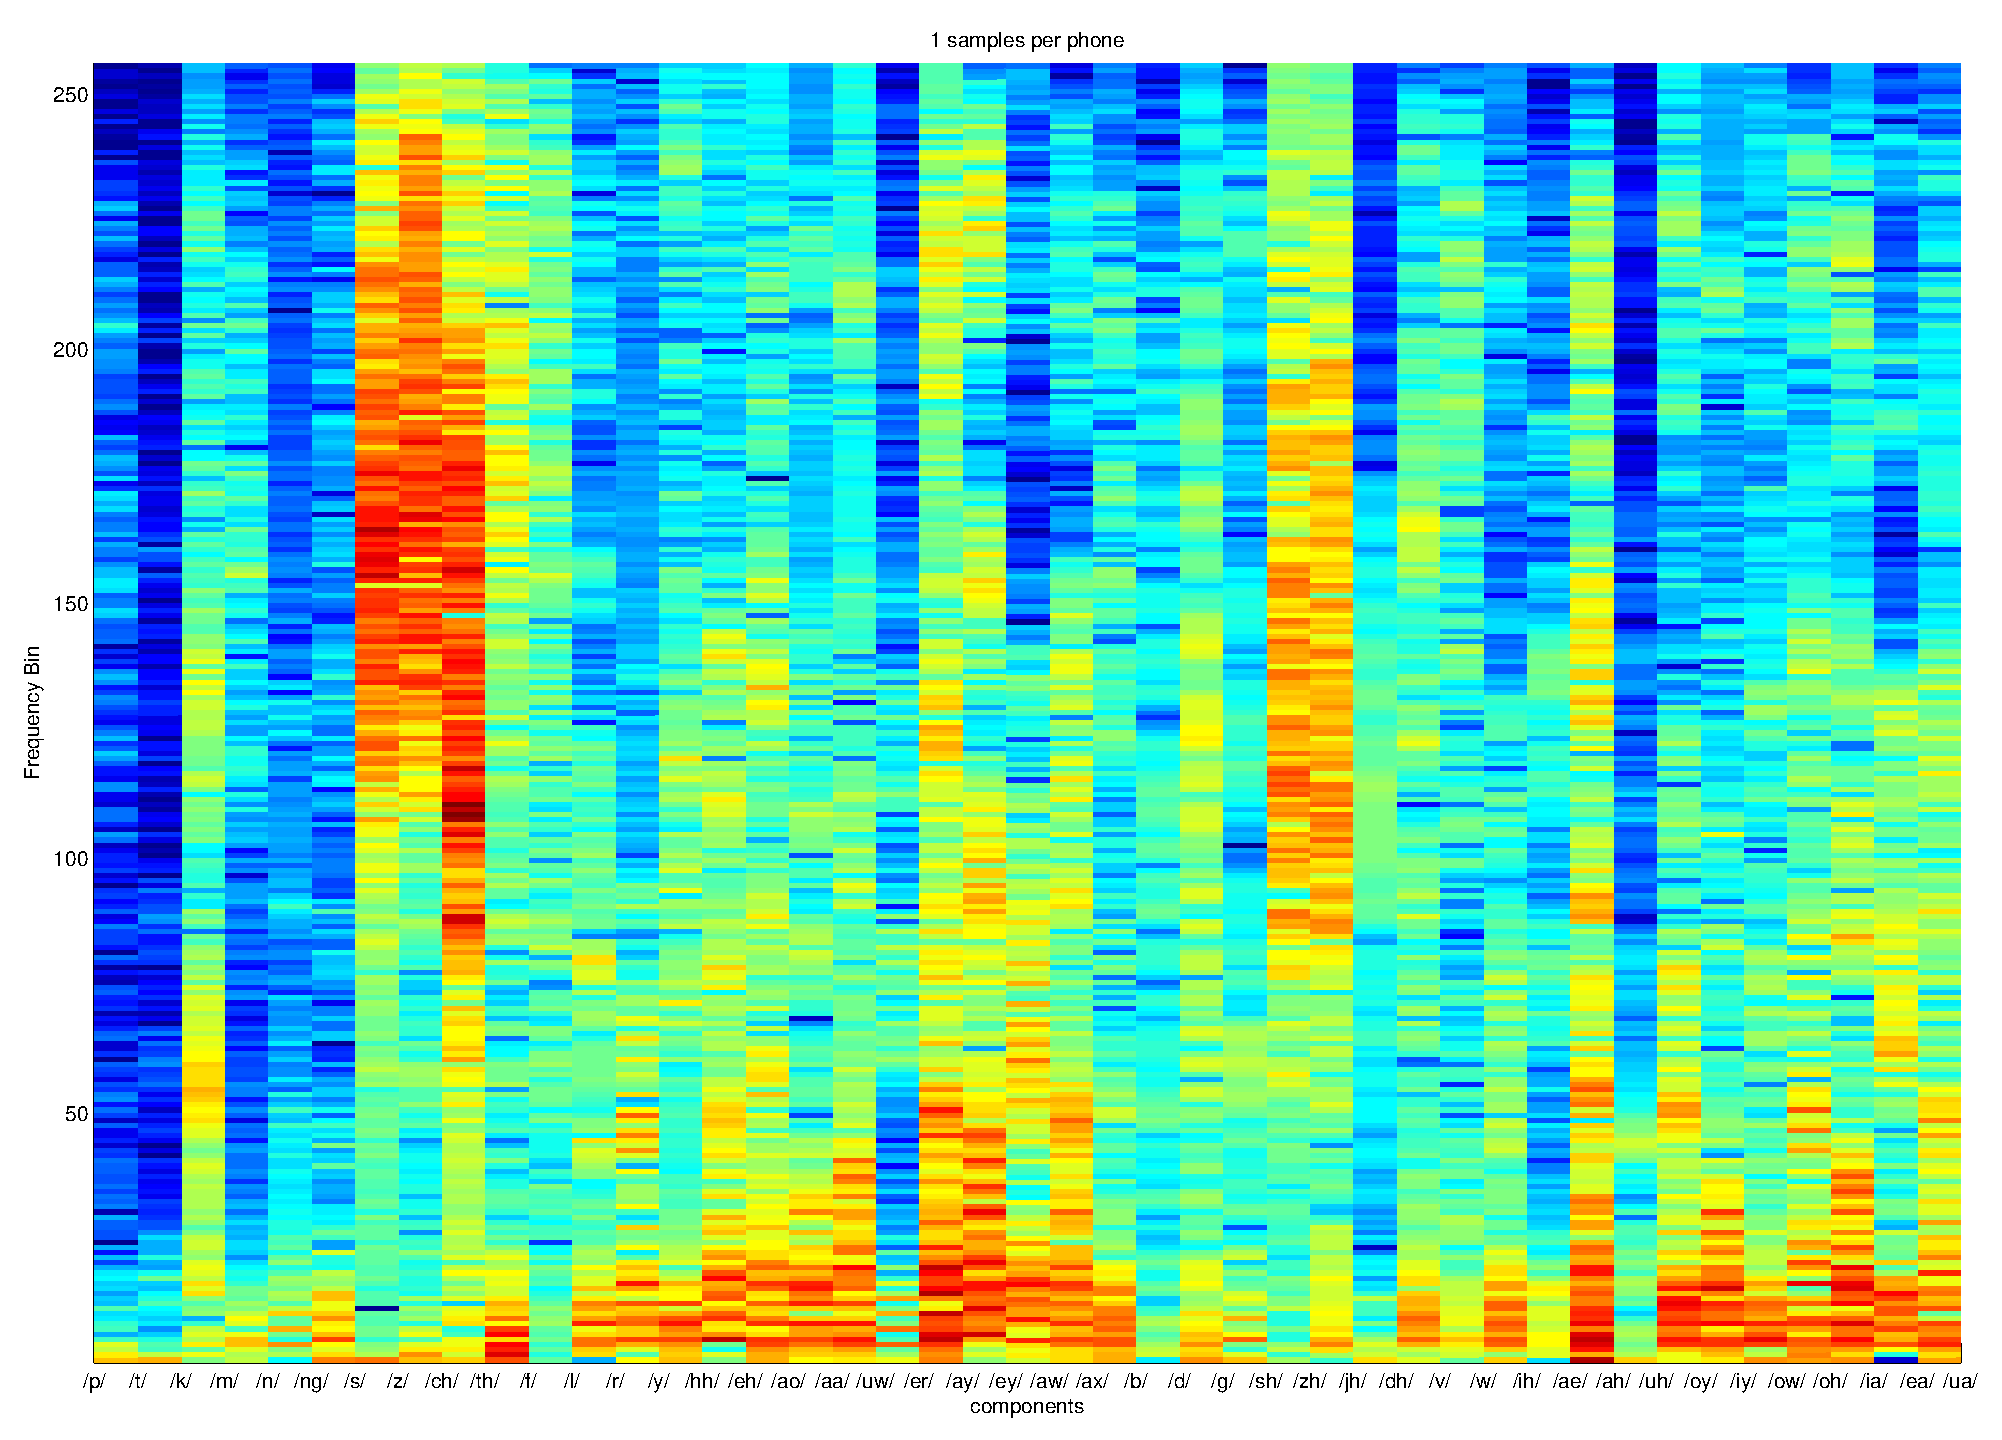
\includegraphics[width=0.5\textwidth]{fig/spectrogram/drawPhn/c3s-1phnSpectrogram}

}\subfloat[\label{fig:mos-comparison-phn-5}Five samples per phoneme]{\includegraphics[width=0.5\textwidth]{fig/spectrogram/drawPhn/c3s-5phnSpectrogram}

}

\subfloat[Ten samples per phoneme]{\includegraphics[width=0.5\textwidth]{fig/spectrogram/drawPhn/c3s-10phnSpectrogram}

}\subfloat[50 samples per phoneme]{\includegraphics[width=0.5\textwidth]{fig/spectrogram/drawPhn/c3s-50phnSpectrogram}

}

\subfloat[100 samples per phoneme]{\includegraphics[width=0.5\textwidth]{fig/spectrogram/drawPhn/c3s-100phnSpectrogram}

}\subfloat[500 samples per phoneme]{\includegraphics[width=0.5\textwidth]{fig/spectrogram/drawPhn/c3s-500phnSpectrogram}

}

\subfloat[999 samples per phoneme]{\includegraphics[width=0.5\textwidth]{fig/spectrogram/drawPhn/c3s-999phnSpectrogram}

}

\protect\caption{\label{fig:drawn-phoneme-spectrogram}Typical spectrogram of randomly
drawn phoneme samples for speaker C3S}
\end{figure}


\begin{figure}[H]
\noindent \begin{centering}
\includegraphics[width=1\textwidth]{fig/R/my/phnCompXY/pesq}
\par\end{centering}

\protect\caption{\label{fig:pesq-comparison-phn}\acs{PESQ} comparison for phoneme-dependent
vs. original enhancement}
\end{figure}


\begin{figure}[H]
\noindent \begin{centering}
\includegraphics[width=1\textwidth]{fig/R/my/phnCompXY/MOS}
\par\end{centering}

\protect\caption{\label{fig:mos-comparison-phn}\acs{MOS} comparison for phoneme-dependent
vs. original enhancement}
\end{figure}


\begin{figure}[H]
\noindent \begin{centering}
\includegraphics[width=1\textwidth]{fig/R/my/phnCompXY/MOSle}
\par\end{centering}

\protect\caption{\label{fig:mosle-comparison-phn}\acs{MOS} listening effort comparison
for phoneme-dependent vs. original enhancement}
\end{figure}


\begin{figure}[H]
\noindent \begin{centering}
\includegraphics[width=1\textwidth]{fig/R/my/phnCompXY/CMOS}
\par\end{centering}

\protect\caption{\label{fig:cmos-comparison-phn}Comparative \acs{MOS} comparison
for phoneme-dependent vs. original enhancement}
\end{figure}


\begin{figure}[H]
\noindent \begin{centering}
\includegraphics[width=1\textwidth]{fig/R/my/phnCompXY/PRRcorr}
\par\end{centering}

\protect\caption{\label{fig:prrcorr-comparison-phn}\acs{PRR} correctness comparison
for phoneme-dependent vs. original enhancement}
\end{figure}


\begin{figure}[H]
\noindent \begin{centering}
\includegraphics[width=1\textwidth]{fig/R/my/phnCompXY/PRRcorrimp}
\par\end{centering}

\protect\caption{\label{fig:prrcorrimp-comparison-phn}\acs{PRR} correctness improvement
comparison for phoneme-dependent vs. original enhancement}
\end{figure}


\begin{figure}[H]
\noindent \begin{centering}
\includegraphics[width=1\textwidth]{fig/R/my/phnCompXY/PRRacc}
\par\end{centering}

\protect\caption{\label{fig:prracc-comparison-phn}\acs{PRR} accuracy comparison for
phoneme-dependent vs. original enhancement}
\end{figure}


\begin{figure}[H]
\noindent \begin{centering}
\includegraphics[width=1\textwidth]{fig/R/my/phnCompXY/PRRaccimp}
\par\end{centering}

\protect\caption{\label{fig:prraccimp-comparison-phn}\acs{PRR} accuracy improvement
comparison for phoneme-dependent vs. original enhancement}
\end{figure}


\begin{figure}[H]
\noindent \begin{centering}
\includegraphics[width=1\textwidth]{fig/R/my/phnCompXY/segSNR}
\par\end{centering}

\protect\caption{\label{fig:segsnr-comparison-phn}Segmental \acs{SNR} comparison
for phoneme-dependent vs. original enhancement}
\end{figure}


\begin{figure}[H]
\noindent \begin{centering}
\includegraphics[width=1\textwidth]{fig/R/my/phnCompXY/segSNRImp}
\par\end{centering}

\protect\caption{\label{fig:segsnrimp-comparison-phn}Segmental \acs{SNR} improvement
comparison for phoneme-dependent vs. original enhancement}
\end{figure}



\subsection{Performance for Humans}

\figref{pesq-comparison-phn} indicated that the phoneme-dependent
\textbf{training} modifications caused, in general, a decline in performance
measured with \ac{PESQ}. The opposite was true, however, for the
phoneme-dependent \textbf{base} modification algorithms. These algorithms
mostly scored higher, with the exceptions mostly belonging the the
NOIZEUS street noise tests.

This is in contrast, however, to the \ac{MOS} results presented in
\cref{fig:mos-comparison-phn,fig:mosle-comparison-phn,fig:cmos-comparison-phn}.
These results did not show any specific pattern of improvement across
different noise types. Thus, results indicated that the phoneme dependence
modifications to these algorithms did not present any significant
improvement for human listeners.

It was noted, however, that the points that did show better enhancement
on the \ac{MOS} scales were more likely to be of the synthetic babble
noise types, \lstinline!c3f(m)! and \lstinline!c3f(m)+c3c(f)+c35(m)!.
These are also associated with the more ``difficult'' forms of noise.
Therefore, it is possible that using phoneme dependence in algorithms
may be useful in source separation applications. This highlights the
ability of phoneme dependence to distinguish between voices, but not
as an efficient method of extracting speech from other noise.

A potential application for such an algorithm is as a second stage
noise cleaning algorithm specifically for competing speaker noise,
or speaker separation. In such a system, another enhancement algorithm
applicable to a broader range of noise types but not for a specific
voice, such as an \ac{MMSE} algorithm, could be used to filter out
non-speech noise, and the phoneme-dependent algorithm then used to
separate the intended voice.


\subsection{Performance for Machines}

The phoneme-dependent \textbf{training} modifications failed to improve
machine correctness almost completely, as indicated in \cref{fig:prrcorr-comparison-phn,fig:prrcorrimp-comparison-phn}.
However, with the exception of the ideal binary mask algorithms and
the \lstinline!c3f(m)! noise type, the phoneme-dependent \textbf{training}
modifications tended to improve the machine correctness. Especially
good performance was noted for the NOIZEUS car noise. This suggested
that using phoneme dependence tended to both increase the algorithm's
ability to remove noise, but also increased the distortion. This observation
was logical, as using phoneme-dependent \textbf{training} was effectively
a way to prevent over-training, so some under-trained characteristics
like this were to be expected.

Potential application for the phoneme-dependent training algorithm
lays in in-car electronics. The algorithms have been shown to improve
for car noise. The NOIZEUS car noise included muffled voices within
the recording.

Interestingly, the increased correctness suggested that the noise
reduction outweighed the distortion for a machine recogniser. The
poor performance for the \lstinline!c3f(m)! noise type was attributed
to the fact that both the \ac{SoI} and the noise were a similar male
voice. The poor performance indicated that phoneme-dependent \textbf{training}
did not particularly aid in separating similar voices. The poor accuracy
was likely due to a high number of false positive phoneme detections,
detected from the second voice.

The phoneme-dependent \textbf{base} modifications showed improvement
in correctness, unlike the phoneme-dependent \textbf{training} modifications,
as best observed in \figref{prrcorr-comparison-phn}. However, in
terms of accuracy, no significant pattern was noted between those
performing better and worse than the original algorithms.

Results indicated, therefore, that the phoneme-dependent methods were
effective in reducing noise, but tended also to distort the speech.
For machines, the noise reduction outweighed the distortion, thereby
increasing the accuracy. However, for humans the distortions may have
been distracting, thereby causing the mixed results.


\subsection{\label{sub:Varying-Phns}Varying the Number of Samples per Phoneme}

\cref{fig:vary-train-phn-pesq,fig:vary-train-phn-mos,fig:vary-train-phn-mosle,fig:vary-train-phn-cmos,fig:vary-train-phn-prrcorr,fig:vary-train-phn-prracc,fig:vary-train-phn-segsnr}
show the \ac{PESQ}, \ac{MOS}, \ac{MOS} listening effort, comparative
\ac{MOS}, \ac{PRR} correctness and \ac{PRR} accuracy results of
the phoneme-dependent enhancement algorithms as a function of the
number of phonemes used in training. These plots are arranged with
the number of trained utterances on the x-axis and test score on the
y-axis. Furthermore, the plots are arranged in a grid with rows corresponding
to the enhancement algorithm used and columns corresponding to the
noise type used in the test. The series colour represents the \ac{SNR}
used for the test data, and dashed lines represent the score of the
dirty signal before enhancement. The R script used to form these plots
is given in \lstref{trainReqPhn}.

\begin{figure}[p]
\noindent \begin{centering}
\includegraphics[width=1\textwidth,height=0.95\textheight,keepaspectratio]{fig/R/trainPh/pesq}
\par\end{centering}

\protect\caption{\label{fig:vary-train-phn-pesq}\acs{PESQ} results of phoneme-dependently
modified algorithms as phoneme training is increased}
\end{figure}


\begin{figure}[p]
\noindent \begin{centering}
\includegraphics[width=1\textwidth,height=0.95\textheight,keepaspectratio]{fig/R/trainPh/MOS}
\par\end{centering}

\protect\caption{\label{fig:vary-train-phn-mos}\acs{MOS} results of phoneme-dependently
modified algorithms as phoneme training is increased}
\end{figure}


\begin{figure}[p]
\noindent \begin{centering}
\includegraphics[width=1\textwidth,height=0.95\textheight,keepaspectratio]{fig/R/trainPh/mosle}
\par\end{centering}

\protect\caption{\label{fig:vary-train-phn-mosle}\acs{MOS} listening effort results
of phoneme-dependently modified algorithms as phoneme training is
increased}
\end{figure}


\begin{figure}[p]
\noindent \begin{centering}
\includegraphics[width=1\textwidth,height=0.95\textheight,keepaspectratio]{fig/R/trainPh/CMOS}
\par\end{centering}

\protect\caption{\label{fig:vary-train-phn-cmos}Comparative \acs{MOS} results of
phoneme-dependently modified algorithms as phoneme training is increased}
\end{figure}


\begin{figure}[p]
\noindent \begin{centering}
\includegraphics[width=1\textwidth,height=0.95\textheight,keepaspectratio]{fig/R/trainPh/prrcorr}
\par\end{centering}

\protect\caption{\label{fig:vary-train-phn-prrcorr} \acs{PRR} correctness results
of phoneme-dependently modified algorithms as phoneme training is
increased}
\end{figure}


\begin{figure}[p]
\noindent \begin{centering}
\includegraphics[width=1\textwidth,height=0.95\textheight,keepaspectratio]{fig/R/trainPh/prracc}
\par\end{centering}

\protect\caption{\label{fig:vary-train-phn-prracc} \acs{PRR} accuracy results of
phoneme-dependently modified algorithms as phoneme training is increased}
\end{figure}


\begin{figure}[p]
\noindent \begin{centering}
\includegraphics[width=1\textwidth,height=0.95\textheight,keepaspectratio]{fig/R/trainPh/segSNR}
\par\end{centering}

\protect\caption{\label{fig:vary-train-phn-segsnr}Segmental \acs{SNR} results of
phoneme-dependently modified algorithms as phoneme training is increased}
\end{figure}


\clearpage{}

\figref{vary-train-phn-pesq} tended to show little correlation between
\ac{PESQ} enhancement and the number of phonemes. However, \cref{fig:vary-train-phn-mos,fig:vary-train-phn-mosle,fig:vary-train-phn-cmos}
tended to show a slight increase in \ac{MOS} performance with the
number of phonemes. However, it was difficult to draw a clear conclusion,
as a smaller number of the tests instead showed a slight decrease.
\figref{my-Corr} agreed with the overall trend of improvement with
increased phoneme samples; showing a slight, yet significant, positive
correlation between \lstinline!phonemes! and \lstinline!MOS!, \lstinline!MOSle!
and \lstinline!CMOS!.

\cref{fig:vary-train-phn-prrcorr,fig:vary-train-phn-prracc} showed,
for most algorithms, no improvement in correctness with increasing
phonemes. However, there was in some cases an increase in accuracy,
especially for \lstinline!phonememodifiedOnline! and \lstinline!phonemeIDBM!,
but rarely a decrease. As above, the significance of the improvement
is low, however a slight positive correlation is present.

For the phoneme-dependent ideal binary mask algorithm (\lstinline!phonemeIDBM!)
there was a clear and significant positive correlation with the number
of phonemes used in training. It was noted that the correctness was
reduced near to zero for one sample per phoneme. For this algorithm,
tests were only performed up to ten samples per phoneme, but it is
likely the performance of these algorithms could have been greatly
improved by using more phoneme samples. 

The correlogram in \figref{my-Corr} showed little correlation between
\lstinline!phonemes! and correctness (\lstinline!PRRcorr!), correctness
improvement (\lstinline!PRRcorrImp!), accuracy (\lstinline!PRRacc!)
and accuracy improvement (\lstinline!PRRaccImp!).

In general, it was found that increasing the number of phonemes drawn
had a chance of improving the performance, for both human and machine
listeners, but had only a low change of decreasing performance and
was very unlikely to severely affect performance. Thus, results indicated
that it would be advantageous to use a higher number samples per phoneme,
an upper bound not having been found.


\subsection{Other Observations}

The performance for the \ac{MMSE} algorithm is unchanged by the introduction
of phoneme-dependence in all of the objective measures, \cref{fig:vary-train-phn-pesq,fig:vary-train-phn-prrcorr,fig:vary-train-phn-prracc,fig:vary-train-phn-segsnr}.
Only in the subjective tests, i.e. the \ac{MOS} tests in \cref{fig:mos-comparison-phn,fig:mosle-comparison-phn,fig:cmos-comparison-phn}
showed variation. This indicated that using phoneme dependence did
not affect the operation of this particular algorithm.

This also highlighted the level of subjectivity involved in the \ac{MOS}
tests, since the scores for the \ac{MMSE} algorithm in \cref{fig:mos-comparison-phn,fig:mosle-comparison-phn,fig:cmos-comparison-phn}
deviated quite significantly from the diagonal line.
